% Created 2016-02-02 Tue 19:21
\documentclass[journal=jpccck,manuscript=article,email=true]{achemso}
  \setkeys{acs}{biblabel=brackets,super=true,articletitle=true}
\SectionNumbersOn
\usepackage[utf8]{inputenc}
\usepackage{fixltx2e}
\usepackage{url}
\usepackage{mhchem}
\usepackage{graphicx}
\usepackage{float}
\usepackage{color}
\usepackage{amsmath}
\usepackage{textcomp}
\usepackage{wasysym}
\usepackage{latexsym}
\usepackage{amssymb}
\usepackage[linktocpage, pdfstartview=FitH, colorlinks, linkcolor=black, anchorcolor=black, citecolor=black, filecolor=black, menucolor=black, urlcolor=black]{hyperref}
\author{John D. Michael}
\author{Ethan L. Demeter}
\author{Steven M. Illes}
\author{Qingqi Fan}
\author{Jacob R. Boes}
\author{John R. Kitchin}
\email{jkitchin@andrew.cmu.edu}
\affiliation{Department of Chemical Engineering, Carnegie Mellon University, 5000 Forbes Ave, Pittsburgh, PA 15213}
\date{}
\title{Alkaline Electrolyte and Fe Impurity Effects on the Performance and Active-phase Structure of NiOOH Thin Films for OER Catalysis Applications}
\begin{document}

\newpage

\begin{abstract}
The effects of varying alkaline electrolyte and electrolyte Fe levels on the performance and active-phase structure of NiOOH thin films for catalysis of the oxygen-evolution reaction (OER) were studied. An electrolyte effect on catalytic performance was observed. Under purified conditions, current densities followed the trend Cs$^{\text{+}}$\textgreater K$^{\text{+}}$$\approx$ Na$^{\text{+}}$$\approx$ Li$^{\text{+}}$ at current densities \textgreater1 mA/cm$^{\text{2}}$. Under Fe-saturated conditions, current densities followed the trend K$^{\text{+}}$$\approx$ Na$^{\text{+}}$\textgreater Cs$^{\text{+}}$\textgreater Li$^{\text{+}}$ at all current densities. Voltammetry was coupled with Raman spectroscopy for studies in LiOH and CsOH. Raman spectra were fit to Gaussian functions and analyzed quantitatively based on mean peak positions. Both purified and Fe-saturated CsOH promoted slightly lower peak positions than purified and Fe-saturated LiOH, indicating that CsOH promoted a NiOOH active-phase structure with longer Ni-O bonds. Both Fe-saturated CsOH and LiOH promoted slightly lower Raman peak positions than purified CsOH and LiOH, but only for one of the two Raman peaks. These results indicate that Fe promoted an active-phase structure with slightly longer Ni-O bonds. This study shows that the catalytic performance and active-phase structure of NiOOH can be tuned by simply varying the alkaline electrolyte and electrolyte Fe levels.
\end{abstract}
\textbf{Keywords} nickel, iron, oxygen evolution, electrochemistry, Raman spectroscopy

\newpage

\section{Introduction}
\label{sec-1}
With a growing global energy demand, the development of clean and renewable platforms for energy storage is a necessity \cite{bard-1995-artif-photos,gray-2009-power,cook-2010-solar-energ}. Electrolysis of water into gaseous hydrogen and oxygen (i.e. \ce{H2O(l)} $\rightarrow$ \ce{H2(g)} + \ce{1/2O2(g)}) has been extensively studied and is considered a feasible technology to meet this energy storage need \cite{dau-2010-mechan-water-oxidat,walter-2010-solar-water,cook-2010-solar-energ}. However, the overpotential needed to drive the oxygen evolution reaction (OER) at a practical rate is a major hindrance to utilization of water-splitting technology for large-scale energy storage \cite{cook-2010-solar-energ}. Metal oxide electrocatalysts have been developed to lower the OER overpotential \cite{dau-2010-mechan-water-oxidat}. Currently, the best performing electrocatalysts are Ru-oxides and Ir-oxides in acidic electrolyte, but the cost and scarcity of these materials renders them impractical for large-scale water electrolysis systems \cite{cook-2010-solar-energ,walter-2010-solar-water,reier-2012-elect-oxygen,mccrory-2013-bench-heter}. Fortunately, earth-abundant and inexpensive Ni$_{\text{1-x}}$Fe$_{\text{x}}$OOH electrocatalysts in alkaline electrolyte have been shown to exhibit comparable performance to Ru-oxide and Ir-oxide electrocatalysts in acidic electrolyte \cite{cook-2010-solar-energ,walter-2010-solar-water,mccrory-2013-bench-heter,smith-2013-water-oxidat-catal,trotochaud-2014-precis}. Ni$_{\text{1-x}}$Fe$_{\text{x}}$OOH readily corrodes in acidic electrolyte, but displays excellent stability in alkaline electrolyte.

Variations in performance of NiOOH OER catalysts have been attributed to differences in active-phase structure \cite{desilvestro-1988-charac-redox,corrigan-1989-elect-spect,yeo-2012-in-situ,bediako-2012-struc-activ}. A recent \emph{in situ} Raman spectroscopy study on NiOOH thin films claimed that repeated cycling of potential converted the thin films from $\gamma$-NiOOH to $\beta$-NiOOH, which corresponded to an increase in catalytic activity  \cite{yeo-2012-in-situ}. An x-ray absorption spectroscopy study on Ni-borate films (comprised on nano-sized domains of NiOOH) concluded that $\gamma$-NiOOH is the more catalytically-active phase \cite{bediako-2012-struc-activ}. Although these studies are contradictory, they clearly show that the active-phase structure of NiOOH is related to performance for OER catalysis.

Fe has been shown to influence active-phase structure and significantly improve the catalytic performance of NiOOH \cite{corrigan-1987-catal-oxygen,landon-2012-spect-charac,louie-2013-inves-thin,smith-2013-water-oxidat-catal,mccrory-2013-bench-heter,trotochaud-2014-nickel-iron}. An \emph{in situ} Raman spectroscopy study showed that variations in Fe content of NiOOH thin film catalysts corresponded to variations in Raman peak positions and peak intensity ratios \cite{louie-2013-inves-thin}. In addition, a recent x-ray absorption spectroscopy study showed that Fe cations are the active sites in Ni$_{\text{1-x}}$Fe$_{\text{x}}$OOH and incorporate into the $\gamma$-NiOOH lattice structure \cite{friebel-2015-ident-highl}. Even unintentional Fe promotion from trace (i.e. ppb) Fe in the stock electrolyte is sufficient to promote the performance of NiOOH for OER catalysis \cite{trotochaud-2014-nickel-iron}. After stock electrolyte was purified of Fe, NiOOH displayed significantly worse catalytic properties \cite{trotochaud-2014-nickel-iron}. OER onset overpotential increased by nearly 150 mV and OER current density at moderate overpotentials decreased significantly \cite{trotochaud-2014-nickel-iron}.

Varying the electrolyte has also been shown to influence catalytic performance. A fuel cell study on Pt electrodes in alkaline electrolyte showed that catalytic activity increased from LiOH to CsOH (i.e. \ce{Cs+}\textgreater\ce{K+}\textgreater\ce{Na+}$\gg$\ce{Li+}) \cite{strmcnik-2009}. Ni-based catalysts for the OER in borate and bicarbonate electrolyte have also been studied, further displaying the synergy between electrolyte choice and catalytic performance \cite{dinca-2010-nickel,bediako-2012-struc-activ,bediako-2013-mechan-studies,joya-2014-ni-based}. An alkaline electrolyte cation effect was shown on \ce{TiO2}-based water-slitting photoanodes where OER current density followed the trend \ce{Li+}\textgreater\ce{Na+}\textgreater\ce{K+} \cite{ding-2015-abnor-effec}. Studies on the \(\ce{Ni(OH)2}/\ce{NiOOH}\) electrode for alkaline battery application have shown that the simple addition of LiOH to KOH with added Fe inhibited ``Fe poisoning" (i.e. reduction in OER overpotentials) \cite{armstrong-1986,kamnev-1996}. In regards to water electrolysis applications, these studies show that KOH is a better alkaline electrolyte than LiOH because it promotes lower OER overpotentials \cite{armstrong-1986,kamnev-1996}. These results suggest that the alkali metal cation trend may continue with CsOH promoting even lower OER overpotentials than LiOH and KOH. Several quartz crystal microbalance (QCM) studies show that alkali cations intercalate and deintercalate during the oxidation and reduction, respectively, of \(\ce{Ni(OH)2}/\ce{NiOOH}\) thin films \cite{barnard-1981-studies-iv,bernard-1991-ac,wehrens-dijksma-2006-elect-quart}. If alkali cations are incorporated into \(\ce{Ni(OH)2}/\ce{NiOOH}\) films, then cations are likely influencing the molecular structure. Since a connection has been shown between active-phase structure and catalytic performance, it is reasonable to hypothesize that varying the alkali hydroxide electrolyte will affect the performance of NiOOH for OER catalysis.

This study is focused on the effects that varying alkaline electrolyte and Fe impurity levels have on the catalytic performance and active-phase structure of NiOOH thin films for OER catalysis. Linear sweep voltammetry (LSV) and \emph{in situ} Raman spectroscopy were used to study catalyst performance and active-phase structure, respectively. Raman spectra were analyzed quantitatively by fitting spectra to a function comprised of Gaussian curves. Due to the effects of trace Fe impurities on catalyst performance, electrolytes were purified before experimentation \cite{trotochaud-2014-nickel-iron}. For some experiments, Fe impurities were re-added to the system in a controlled manner. This study showed a cation effect on catalytic performance in purified and Fe-saturated electrolyte. In purified electrolyte, current density followed the trend Cs$^{\text{+}}$\textgreater K$^{\text{+}}$\textgreater Na$^{\text{+}}$$\approx$ Li$^{\text{+}}$ at appreciable current densities. In Fe-saturated electrolyte, current density followed the trend K$^{\text{+}}$$\approx$ Na$^{\text{+}}$\textgreater Cs$^{\text{+}}$\textgreater Li$^{\text{+}}$. Adding Fe impurities shifted the trend in catalytic performance such that Fe-saturated KOH and NaOH promoted the best catalytic performance for NiOOH. LSV was coupled with \emph{in situ} Raman spectroscopy to determine trends between active-phase structure and catalytic performance in LiOH and CsOH. CsOH promoted lower peak positions than LiOH for both the O-Ni-O bending and stretching modes in purified and Fe-saturated electrolyte. In addition, Fe-saturated electrolyte promoted a slightly lower peak position for the O-Ni-O bending mode in comparison to purified electrolyte. These results indicate that differences in OER catalytic performance between purified and Fe-saturated LiOH and CsOH can be attributed to differences in the active-phase structure of NiOOH for OER catalysis.

\section{Methods}
\label{sec-2}
\subsection{Electrolyte and Thin Film Preparation}
\label{sec-2-1}
Experiments were performed in 0.1 M electrolyte prepared from high-purity LiOH (Sigma-Aldrich), NaOH (Fluka), KOH (Fluka), and CsOH (Sigma-Aldrich). Experiment were primarily conducted in LiOH and CsOH. Ultrapure water ($\approx$18 M$\Omega$) was used during all experiments. Electrolytes were purified of trace Fe by soaking 1 M electrolyte with Ni(OH)$_{\text{2}}$ (i.e. Fe adsorbent) in a polypropylene vial for at least 12 hours \cite{trotochaud-2014-nickel-iron}. Ni(OH)$_{\text{2}}$ was prepared for Fe adsorption by combining $\approx$2 g of high-purity \(\ce{Ni(NO3)2}\) (Sigma-Aldrich) with 20 mL of 1 M LiOH, NaOH, KOH, or CsOH. Precipitation of  Ni(OH)$_{\text{2}}$ occurred immediately. Images of the apparatus for electrolyte purification can be found in Supporting Information. For experiments with Fe added to purified electrolyte, a 4000 ppm \(\ce{Fe(NO3)3}\) (Sigma-Aldrich) solution was prepared with ultrapure water. \(\ce{Fe(NO3)3}\) solution was diluted in 0.1 M electrolyte to $\approx$1 ppm. The final concentration of Fe in the electrolyte was approximate since precipitation of \(\ce{Fe(OH)2}\) occurred, indicating saturation.

Electrochemical experiments were performed with a Gamry Reference 600 potentiostat/galvanostat and a compact, three-electrode system (Pine Instruments). The three-electrode system consisted of a Au working electrode (diameter=2 mm), Au counter electrode, and Ag/AgCl reference electrode (RE). Geometric surface area of the working electrode was used for all current density calculations. An external Hg/HgO RE (Koslow Scientific Company) was used in place of the Ag/AgCl RE for experiments in alkaline electrolyte. The Hg/HgO reference electrode was calibrated against a Hg/HgO "lab master" reference electrode for each experiment. Both the experimental and "lab master" reference electrodes were filled with 0.1 M KOH and were stored in 0.1 M KOH within a sealed container, to minimize drifts in potential. Images of the three-electrode system and electrochemical cells can be found in Supporting Information. Prior to electrodeposition, the Au working electrode was electrochemically roughened in \(\ce{H2SO4}\) (0.5 M) with cyclic voltammetry (CV) from -0.2 - 1.3 V (vs. Ag/AgCl) at 60 mV/s. Ni(OH)$_{\text{2}}$ was electrodeposited from an unstirred 0.01 M \(\ce{Ni(NO3)2}\) solution onto the Au working electrode at -0.8 mA/cm$^{\text{2}}$ for 10 seconds. To estimate Ni loading, Gamry potentiostat/galvanostat software was used to integrate the area under the Ni(OH)$_{\text{2}}$/NiOOH redox peaks in the voltammetry data. This integration yielded a charge of $\approx$150 uC. This was consistent throughout all experiments, since the same electrodeposition technique was used to prepare all Ni(OH)$_{\text{2}}$/NiOOH thin films. Assuming a one-electron transfer during redox, $\approx$150 \textmu{}C corresponded to $\approx$1.55\texttimes{}10$^{\text{-9}}$ mol Ni$^{\text{2+/3+}}$ on the working electrode surface. Furthermore, the film thickness was $\approx$30 nm based on results in a recent Ni(OH)$_{\text{2}}$/NiOOH OER study \cite{trotochaud-2014-nickel-iron}

\subsection{Voltammetry with Electrolyte Switching}
\label{sec-2-2}
Voltammetry was performed while switching the electrolyte between LiOH and CsOH or NaOH and KOH. This was done to compare catalytic performance and test the reversibility of the electrolyte cation effect on catalytic performance. After electrodeposition, CV was performed from 0.2 - 0.8 V (vs. Hg/HgO) at 50 mV/s in LiOH, for example, until CV curves stabilized ($\approx$60 cycles). LSV was then performed from 0.2 - 0.9 V (vs. Hg/HgO) at 1 mV/s in LiOH. Electrolyte was replaced with CsOH, for example, and the experiment was repeated. Studies were performed in purified and Fe-saturated electrolyte. The reverse procedure was performed and yielded nearly identical results. The reverse procedure is actually captured within the original procedure, since the electrolytes were switched several times for a single electrode. The same procedure was applied to NaOH and KOH. Results from experiments in NaOH and KOH can be found in Supporting Information. Results of a Tafel analysis on LSV curves in purified and Fe-saturated LiOH, NaOH, KOH, and CsOH can also be found in Supporting Information.

It was determined that correcting voltammetry data for iR was not necessary due to the small magnitude of iR relative to overpotential. The small magnitude arose from 1) all electrolytes being sufficiently conductive due to the concentrated electrolyte used (0.1 M), 2) the reference electrode and working electrode being closely and consistently spaced ($\approx$1 cm.), 3) all experiments being performed on thin films, which according to literature do not significantly influence iR, and 4) the working electrode substrate and counter electrode being Au \cite{trotochaud-2014-precis}.
An approximate iR of $\approx$4.0\texttimes{}10$^{\text{-7}}$ mV was calculated at the highest observed current (8.47\texttimes{}10$^{\text{-4}}$ A) for 0.1 M KOH at 25$^{\circ{}}$C based on the reference and working electrode spacing ($\approx$ 1 cm.) and specific conductivity (2.13\texttimes{}10$^{\text{6}}$ S/cm) from the CRC Handbook \cite{crc-95}. Although this value of iR is an approximation, it is several orders of magnitude less than the overpotentials observed in this study. iR at lower currents would be even smaller. Since specific conductivity for LiOH, NaOH, KOH, and CsOH does not differ significantly at 0.1 M and 25$^{\circ{}}$C and all electrolytes were prepared the same way, different series resistances for each electrolyte were assumed to be insignificant.

\subsection{Voltammetry with in situ Raman Spectroscopy}
\label{sec-2-3}
Voltammetry was coupled with \emph{in situ} Raman spectroscopy to study the active-phase structure of \(\ce{Ni(OH)2}/\ce{NiOOH}\) under OER conditions. This experiment was only performed in LiOH and CsOH. After electrodeposition, CV was performed from 0.2 - 0.8 V (vs. Hg/HgO) at 50 mV/s in LiOH until CV curves stabilized ($\approx$60 cycles). LSV was then performed from 0.2 - 0.9 V (vs. Hg/HgO) at 1 mV/s. During LSV, Raman spectra were collected at a range of overpotentials where OER was occurring. Spectra were also collected when the film was in a reduced state (i.e. Ni(OH)$_{\text{2}}$) and OER was not occurring (see Supporting Information). Studies were conducted in purified and Fe-saturated electrolyte.

\emph{In situ} Raman spectroscopy was performed with a Horiba LabRAM HR Raman microscope, Olympia 50x LWD objective, and CCD detector. Laser excitation came from a Spectra-Physics Millenia Pro Nd:YAG laser (wavelength=532 nm). Spectra were collected from 250 cm$^{\text{-1}}$ - 750 cm$^{\text{-1}}$ with laser power at 20 mW, exposure time at 5 seconds, and an accumulation number of 5. A custom electrochemical cell (see Supporting Information) was used so that the compact, three-electrode system could be interfaced with the Raman spectroscopy system. Raman spectra were fit to a function comprised of several Gaussian curves (see Supporting Information) and analyzed based on average peak positions.

\section{Results and Discussion}
\label{sec-3}
\subsection{LSV with Electrolyte Switching}
\label{sec-3-1}
Figure \ref{fig-1} shows the results of LSV on a NiOOH thin film while switching the electrolyte between purified CsOH, KOH, NaOH, and LiOH (all at 0.1 M). Figures showing the separate results of LSV in purified LiOH/CsOH (Figure S1) and NaOH/KOH (Figure S2) can be found in Supporting Information.

\begin{figure}[h]
\centering
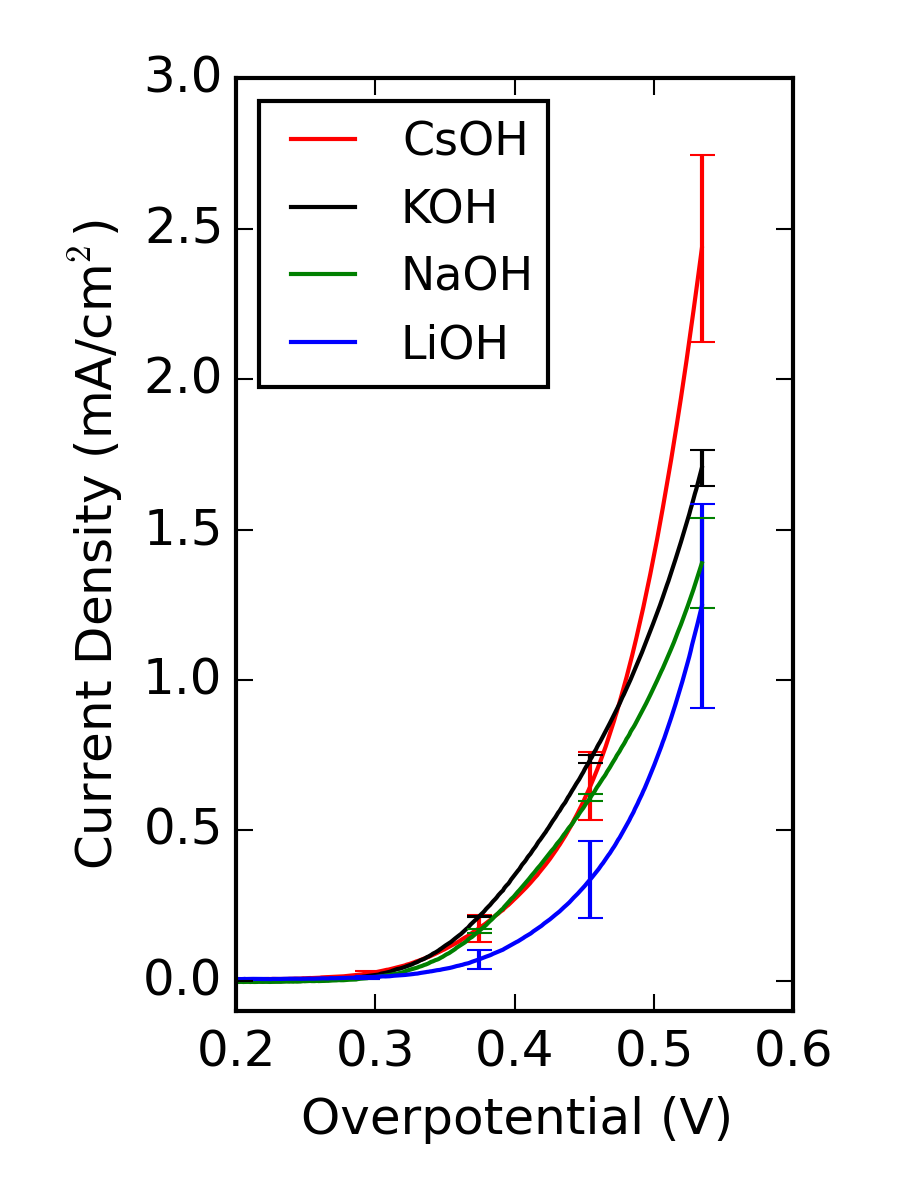
\includegraphics[width=3in]{./images/figures-main/IvsV-Na-K-Li-Cs-pure.png}
\caption{\label{fig-1}LSV of NiOOH in purified LiOH (blue), NaOH (green), KOH (black), and CsOH (red). Potential was swept at 1 mV/s. Error bars represent one standard deviation from mean current density at each respective potential.}
\end{figure}

A cation effect on NiOOH catalyst performance was observed in purified electrolyte. CsOH promoted approximately double the OER current density of LiOH trials at all potentials where appreciable OER occurred. For example, at an overpotential of 0.5 V the OER current density in LiOH was $\approx$0.5 mA/cm$^{\text{2}}$ and the OER current density in CsOH was $\approx$1 mA/cm$^{\text{2}}$. KOH promoted slightly higher current densities than NaOH and CsOH from the onset of OER until $\approx$0.45 V. Beyond overpotentials of $\approx$0.45 V, catalytic performance followed the trend of Cs$^{\text{+}}$\textgreater K$^{\text{+}}$$\approx$ Na$^{\text{+}}$$\approx$ Li$^{\text{+}}$. However, the only unambiguous trend was that CsOH promoted higher OER current densities than LiOH at all overpotentials where appreciable OER was occurring. LSV was coupled with Raman spectroscopy in purified LiOH and CsOH to explore the connection between active-phase structure and catalytic performance.

Figure \ref{fig-2} shows the results of LSV on NiOOH while switching the electrolyte between Fe-saturated KOH, NaOH, CsOH, and LiOH (all at 0.1 M). Figures showing the results of LSV in Fe-saturated LiOH/CsOH (Figure S3) and NaOH/KOH (Figure S4) can be found in Supporting Information.

\begin{figure}[h]
\centering
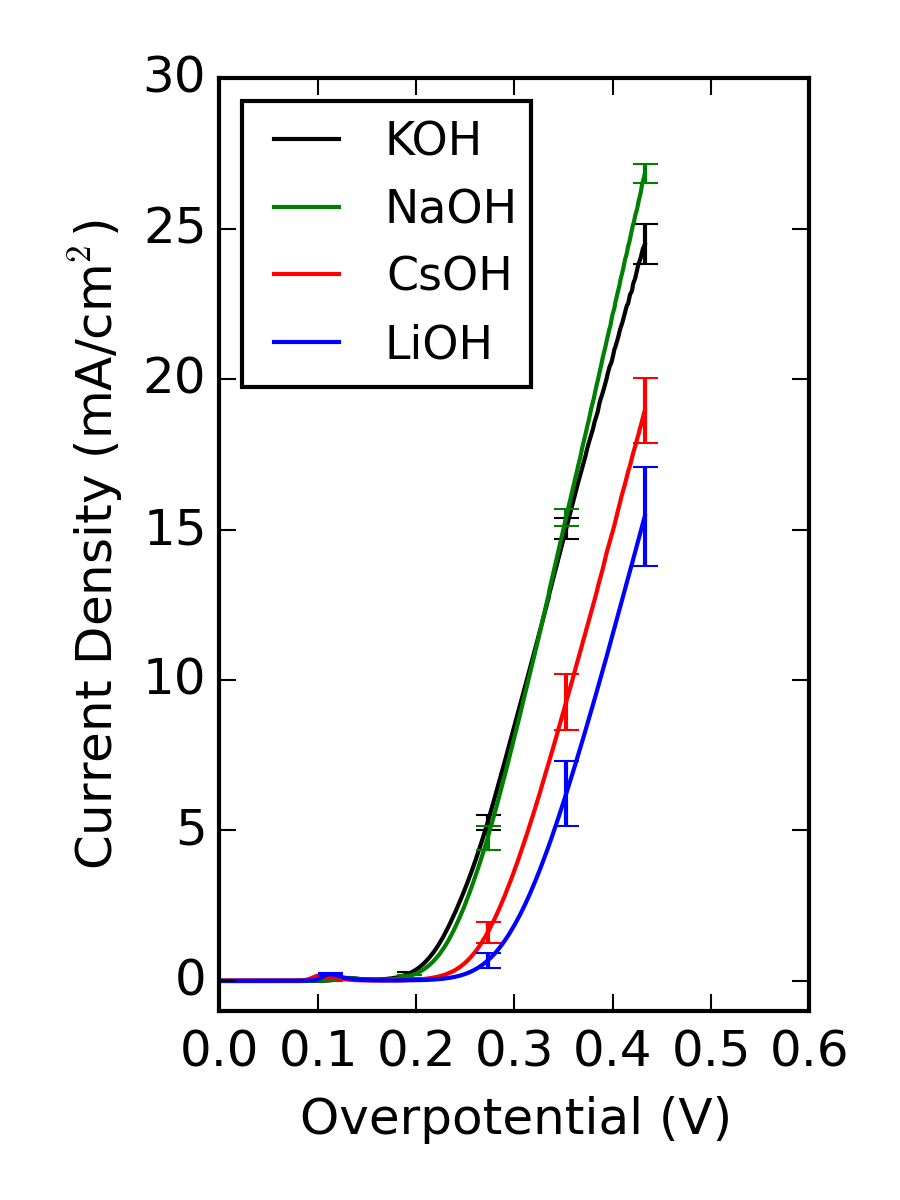
\includegraphics[width=3in]{./images/figures-main/IvsV-Na-K-Li-Cs-iron.png}
\caption{\label{fig-2}LSV of NiOOH in Fe-saturated KOH (black), NaOH (green), CsOH (red), and LiOH (blue). Potential was swept at 1 mV/s. Error bars represent one standard deviation from mean current density at each respective potential.}
\end{figure}

A cation effect on NiOOH catalyst performance was also observed in Fe-saturated electrolyte. However, Fe-saturated KOH and NaOH promoted significantly higher OER current densities than CsOH and LiOH. For example, at an overpotential of 0.3 V, KOH and NaOH promoted a current density of $\approx$7 mA/cm$^{\text{2}}$, CsOH promoted a current density of $\approx$4.5 mA/cm$^{\text{2}}$, and LiOH promoted a current density of $\approx$2.5 mA/cm$^{\text{2}}$. LSV curves for NaOH and KOH overlap until $\approx$0.4 V. Current density likely diverged between NaOH and KOH from differences in oxygen bubble coverage on the working electrode surface, causing a hindrance to the passage of current. In addition, the same trend in catalytic performance observed in purified CsOH and LiOH was also observed in Fe-saturated LiOH and CsOH. CsOH promoted an $\approx$50\% higher OER current density than LiOH at all overpotentials where appreciable OER occurred. LSV was coupled with Raman spectroscopy in Fe-saturated LiOH and CsOH to explore the connection between active-phase structure and catalytic performance. LiOH and CsOH were chosen because the trend of CsOH \textgreater LiOH was observed in both purified and Fe-saturated electrolyte.

Comparing Figures \ref{fig-1} and \ref{fig-2}, the addition of a relatively small amount of \(\ce{Fe(NO3)3}\) to the electrolyte had huge effects on catalytic performance. OER onset overpotential decreased by at least 100 mV in all four electrolytes. Furthermore, OER current density increased by nearly an order of magnitude in all four electrolytes. Under purified conditions, KOH and NaOH promoted intermediate OER current densities. However, under Fe-saturated conditions KOH and NaOH promoted OER current densities that clearly exceeded the catalytic performance promoted by both LiOH and CsOH. Thus, Fe interacted with KOH and NaOH in a way that further promoted the catalytic performance of NiOOH. A recent study by Trotochaud et al. was used to approximate the Fe content of thin films in all electrolytes based on the relative position of the Ni redox peak \cite{trotochaud-2014-nickel-iron}. All redox peaks in purified electrolyte resembled the redox peak in purified electrolyte from the referenced study \cite{trotochaud-2014-nickel-iron}. All redox peaks in Fe-saturated electrolyte resembled the redox peaks of films with an Fe content between 5\% and 25\% from the referenced study \cite{trotochaud-2014-nickel-iron}. More precise Fe content characterization was not necessary for films in Fe-saturated electrolyte since the referenced study showed nearly identical catalytic performance (i.e. OER curves overlapped) for Ni$_{\text{1-x}}$Fe$_{\text{x}}$OOH films with 5\% Fe and 25\% Fe \cite{trotochaud-2014-nickel-iron}. Even if KOH and NaOH promoted higher Fe uptake than CsOH or LiOH, the differences in Fe content are not significant enough to justify the differences in catalytic performance.

Overall the ``cation effect" was small in comparison to the effects of saturating the electrolyte with Fe. However, these results clearly show that a ``double-promotion" effect on NiOOH thin films can be attained for OER catalysis. That is, the catalytic performance of NiOOH can be tuned by simply varying Fe-levels and alkaline electrolyte.
\subsection{LSV with in situ Raman spectroscopy}
\label{sec-3-2}
Figure \ref{fig-3} shows Raman spectra on NiOOH collected during LSV at overpotentials of 240, 340, and 440 mV in purified LiOH (blue) and CsOH (black). LSV results that accompany the spectra in Figure \ref{fig-3} can be found in Supporting Information (Figure S5). According to Figure S5, overpotentials of 240, 340, and 440 mV corresponded to current densities of 0, $\approx$0.5, and $\approx$2.5 mA/cm$^{\text{2}}$ in LiOH and 0, $\approx$1.5, and $\approx$4.0 mA/cm$^{\text{2}}$ in CsOH, respectively. In Figure \ref{fig-3}, red curves represent Gaussian functions that were fit to spectra data. Black vertical lines were included at Raman shifts of 480 cm$^{\text{-1}}$ and 560 cm$^{\text{-1}}$ for easier comparison of spectra. Peaks at $\approx$480 cm$^{\text{-1}}$ correspond to O-Ni-O bending modes and peaks at $\approx$560 cm$^{\text{-1}}$ correspond to O-Ni-O stretching modes \cite{desilvestro-1988-charac-redox}. To accompany Figure \ref{fig-3}, Table \ref{tab:1} shows average Raman peak positions in purified LiOH and CsOH, as determined from the Gaussian functions that were fit to Raman spectra.

\begin{figure}[h]
\centering
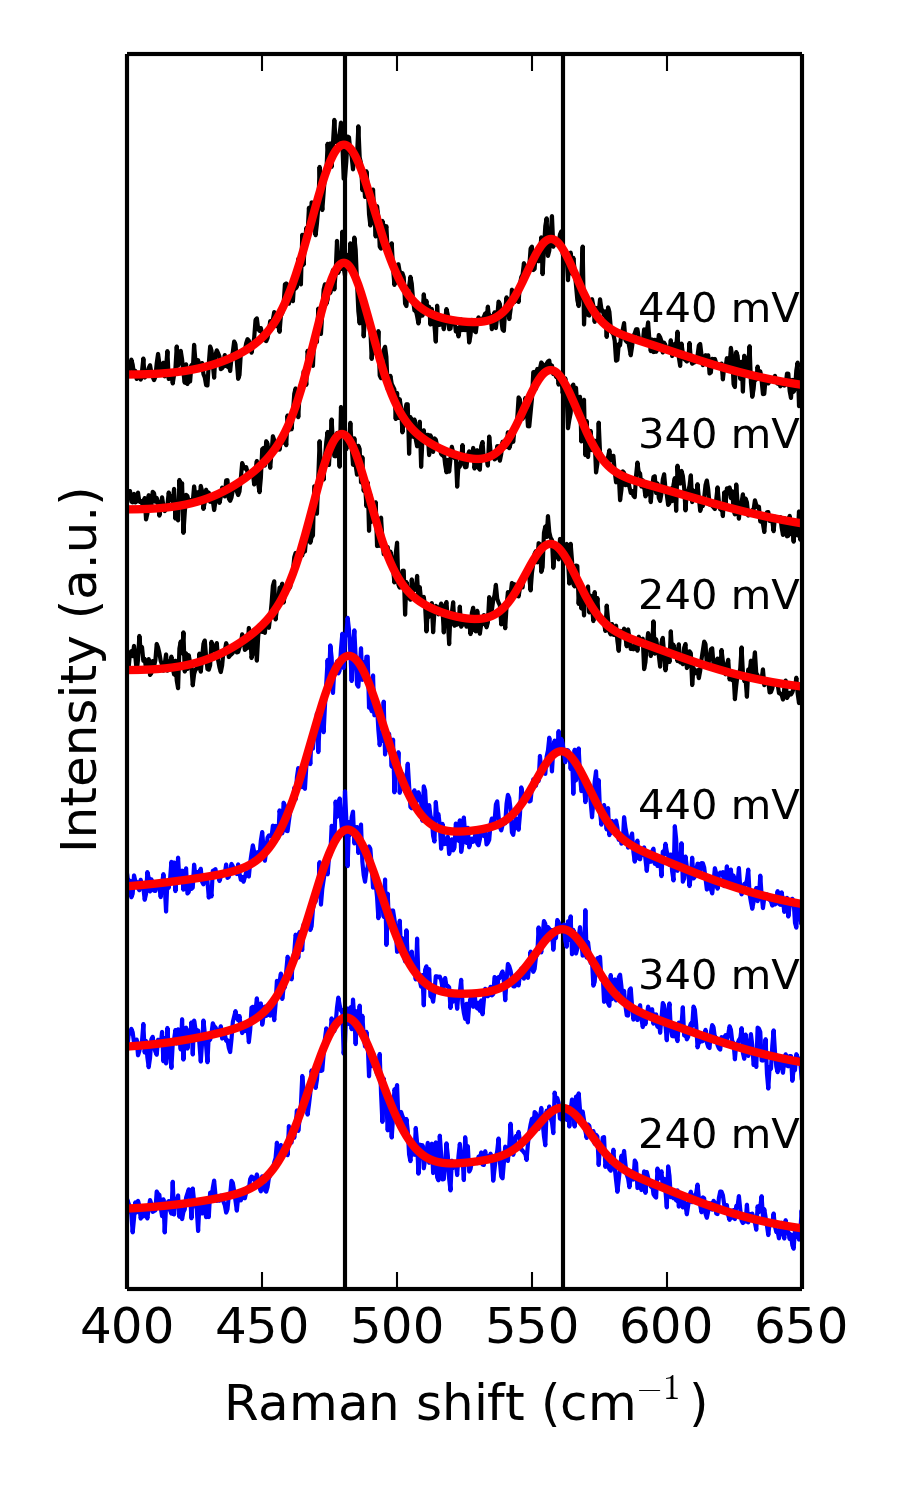
\includegraphics[width=3in]{./images/figures-main/raman-combined-pure-10-31-14.png}
\caption{\label{fig-3}Raman spectra during LSV at overpotentials of 240, 340, 440 mV in purified LiOH (blue, lower three) and CsOH (black, upper three). Red curves represent Gaussian functions that were fit to spectra data. The black lines correspond to 480 cm$^{\text{-1}}$ and 560 cm$^{\text{-1}}$, which are the approximate Raman shifts for the O-Ni-O bending and stretching modes, respectively.}
\end{figure}

\begin{table}[h]
\caption{\label{tab:1}Average Raman peak positions at overpotentials of 240, 340, and 440 mV in purified LiOH and CsOH. Left peaks correspond to O-Ni-O bending modes and right peaks correspond to O-Ni-O bending modes.}
\centering
\begin{tabular}{| c | c | c | c |}
\hline
\textbf{Overpotential=} & \textbf{240 mV} & \textbf{340 mV} & \textbf{440 mV}\\
\hline
LiOH, left peak & 480.43 \textpm \enspace 0.23 & 480.93 \textpm \enspace 0.20 & 481.27 \textpm \enspace0.19\\
\hline
CsOH, left peak & 478.87 \textpm \enspace 0.17 & 479.47 \textpm \enspace 0.15 & 479.77 \textpm \enspace 0.15\\
\hline
LiOH, right peak & 562.07 \textpm \enspace 0.51 & 561.93 \textpm \enspace 0.47 & 561.13 \textpm \enspace 0.39\\
\hline
CsOH, right peak & 557.03 \textpm \enspace 0.35 & 556.93 \textpm \enspace 0.27 & 556.57 \textpm \enspace 0.26\\
\hline
\end{tabular}
\end{table}

Figure \ref{fig-3} shows that both peaks for CsOH exhibited slightly lower Raman shifts compared to both peaks for LiOH at all three overpotentials. Table \ref{tab:1} further supports this claim, showing that both peaks for CsOH had lower average peaks positions than LiOH by $\approx$1.5 cm$^{\text{-1}}$ and $\approx$5.0 cm$^{\text{-1}}$, respectively. These results indicate that purified CsOH and LiOH promoted different NiOOH active-phase structures. In addition, average peak position did not change significantly with increasing overpotential. According to Hardcastle and Wachs, a lower Raman peak position corresponds to longer metal-oxygen bonds \cite{hardcastle-1990-deter-raman}. With \emph{in situ} Raman spectra alone and inconsistencies between the interpretation of Raman spectra of NiOOH in literature, a structural designation cannot be unambiguously assigned for NiOOH from results in this study \cite{cornilsen-1990-struc,yeo-2012-in-situ,louie-2013-inves-thin}. However, purified CsOH promoted a NiOOH active-phase structure with longer Ni-O bonds than purified LiOH. Longer Ni-O bonds corresponded to higher OER current densities, indicating a correlation between active-phase structure and catalytic performance.

Figure \ref{fig-4} shows Raman spectra collected during LSV at overpotentials of 240, 340, and 440 mV in Fe-saturated LiOH (blue) and CsOH (black). LSV results that accompany the spectra in Figure \ref{fig-4} can be found in Supporting Information (Figure S6). According to Figure S6, overpotentials of 240, 340, and 440 mV corresponded to current densities of $\approx$1.0, $\approx$4.0, and $\approx$7.5 mA/cm$^{\text{2}}$ in LiOH and $\approx$2.0, $\approx$5, and $\approx$10.5 mA/cm$^{\text{2}}$ in CsOH, respectively. To accompany Figure \ref{fig-4}, Table \ref{tab:1} shows average Raman peak positions in Fe-saturated LiOH and CsOH.

\begin{figure}[htb]
\centering
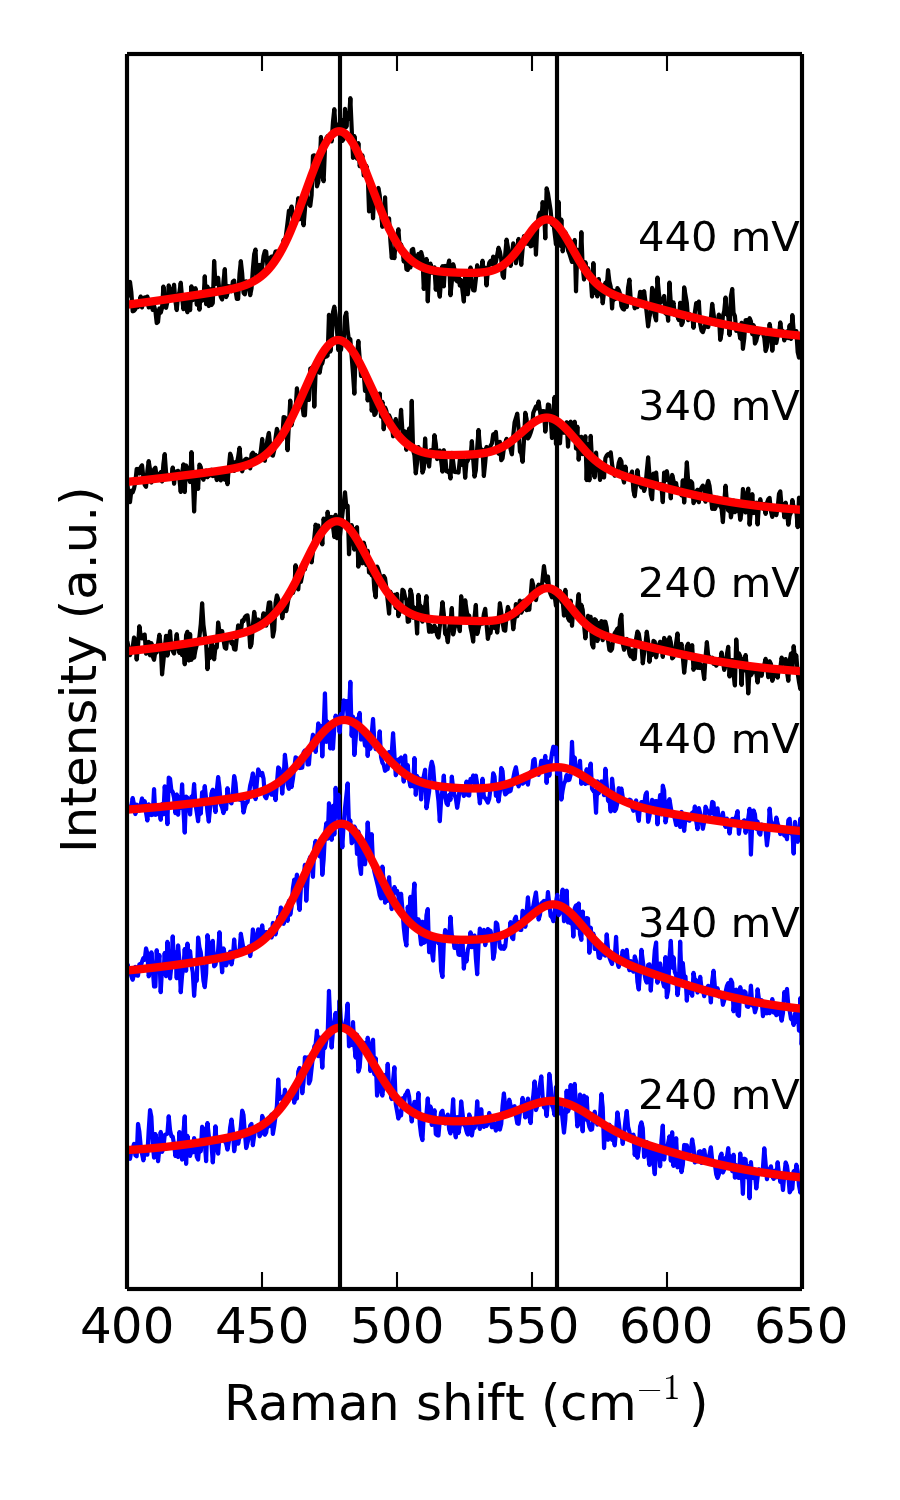
\includegraphics[width=3in]{./images/figures-main/raman-combined-Fe-11-19-14.png}
\caption{\label{fig-4}Raman spectra during LSV at overpotentials of 240, 340, 440 mV in Fe-saturated LiOH (blue, lower three) and CsOH (black, upper three). Red curves represent Gaussian functions that were fit to spectra data. The black lines correspond to 480 cm$^{\text{-1}}$ and 560 cm$^{\text{-1}}$, which are the approximate Raman shifts for the O-Ni-O bending and stretching modes, respectively.}
\end{figure}

\begin{table}[htb]
\caption{\label{tab:2}Average Raman peak positions at overpotentials of 240, 340, and 440 mV in Fe-saturated LiOH and CsOH. Left peaks correspond to O-Ni-O bending modes and right peaks correspond to O-Ni-O stretching modes.}
\centering
\begin{tabular}{| c | c | c | c |}
\hline
\textbf{Overpotential=} & \textbf{240 mV} & \textbf{340 mV} & \textbf{440 mV}\\
\hline
LiOH, left peak & 479.03 \textpm \enspace 0.35 & 479.87 \textpm \enspace 0.40 & 479.93 \textpm \enspace 0.37\\
\hline
CsOH, left peak & 477.53 \textpm \enspace 0.31 & 478.37 \textpm \enspace 0.32 & 478.13 \textpm \enspace 0.30\\
\hline
LiOH, right peak & 559.83 \textpm \enspace 0.84 & 560.60 \textpm \enspace 0.95 & 560.17 \textpm \enspace 0.83\\
\hline
CsOH, right peak & 554.97 \textpm \enspace 0.73 & 556.07 \textpm \enspace 0.64 & 556.30 \textpm \enspace 0.63\\
\hline
\end{tabular}
\end{table}

Figure \ref{fig-4} shows that both peaks for CsOH exhibited slightly lower Raman shifts compared to both peaks for LiOH at all three overpotentials. Table \ref{tab:2} supports this claim, showing that both peaks for CsOH had lower average peaks positions than LiOH by $\approx$1.5 cm$^{\text{-1}}$ and $\approx$4.5 cm$^{\text{-1}}$, respectively. Thus, Fe-saturated CsOH promoted an active-phase structure with longer Ni-O bonds compared to Fe-saturated LiOH \cite{hardcastle-1990-deter-raman}. In addition, average peak position did not change significantly with increasing overpotential. As mentioned before, a structural designation is difficult to make with Raman spectra results alone and discrepancies between the interpretation of Raman spectra in literature \cite{cornilsen-1990-struc,yeo-2012-in-situ,louie-2013-inves-thin}. However, Fe-saturated CsOH promoted a NiOOH active-phase structure with longer Ni-O bonds than Fe-saturated LiOH. Longer Ni-O bonds corresponded to higher OER current densities, further indicating a correlation between active-phase structure and catalytic performance.

A cation effect on the catalytic performance and active-phase structure of NiOOH thin films for OER catalysis was observed in both purified and Fe-saturated LiOH and CsOH. In Figures S5 and S6, purified and Fe-saturated CsOH promoted a significantly larger OER current density than purified and Fe-saturated LiOH, respectively. Comparing the results in Tables \ref{tab:1} and \ref{tab:2}, Fe-saturated electrolyte promoted slightly lower ($\approx$1cm$^{\text{-1}}$) Raman peak positions than purified electrolyte for the left peaks at all three overpotentials in LiOH and CsOH. However, a significant difference between average position of the right peaks was not observed between Fe-saturated and purified electrolyte at any of the three overpotentials in LiOH and CsOH. These results indicate that Fe had a much smaller effect on Raman-sensitive NiOOH structural features in comparison to CsOH. It was recently shown that Fe occupies Ni positions within the NiOOH lattice and is actually the active site for OER catalysis \cite{friebel-2015-ident-highl}. Thus, Fe-saturated electrolyte likely promoted OER catalysis from more active sites being present. The recent study also showed that Fe had a small influence on Ni-O bond distance, which is consistent with the small differences between Raman shift ($\approx$1 cm$^{\text{-1}}$) in purified and Fe-saturated electrolyte \cite{friebel-2015-ident-highl}. However, the precise mechanism by which CsOH promoted better catalytic performance than LiOH is unclear with results from this study. The longer Ni-O bonds may correspond to a more open NiOOH lattice, yielding more facile transport to and from OER active sites.

Although a structural designation is unambiguous with only Raman spectroscopy results, a clear trend between Ni-O bond length and catalytic performance was observed. Lower Raman shifts (i.e. longer Ni-O bond lengths) corresponded to higher OER current densities, indicating a relationship between active-phase structure and catalytic performance \cite{hardcastle-1990-deter-raman}. Furthermore, these results indicate that both catalytic performance and active-phase structure can be tuned by simply altering the electrolyte environment.

\section{Conclusions}
\label{sec-4}
In this study, linear sweep voltammetry (LSV) and \emph{in situ} Raman spectroscopy were used to study the effects of varying alkaline electrolyte conditions on catalytic performance and active-phase structure of NiOOH thin films for OER catalysis. Studies were conducted in purified and Fe-saturated LiOH, NaOH, KOH, and CsOH. Results from LSV showed a cation effect on NiOOH OER catalysis. In purified electrolyte, OER current density showed a trend of Cs$^{\text{+}}$\textgreater K$^{\text{+}}$$\approx$ Na$^{\text{+}}$$\approx$ Li$^{\text{+}}$ at current densities above $\approx$1 mA/cm$^{\text{2}}$. With overlap between some errors bars, the only unambiguous conclusion is that purified CsOH promoted current densities that were $\approx$100\% higher than current densities promoted by purified LiOH. In contrast, Fe-saturated electrolyte promoted a trend in current density of K$^{\text{+}}$$\approx$ Na$^{\text{+}}$\textgreater Cs$^{\text{+}}$\textgreater Li$^{\text{+}}$ at all current densities. Current densities in Fe-saturated KOH and NaOH were $\approx$50\% higher than current densities in Fe-saturated CsOH and $\approx$150\% higher than current densities in Fe-saturated LiOH. Thus, adding Fe to the electrolyte caused an undefined interaction with KOH and NaOH, likely within the NiOOH lattice, that promoted the highest current densities observed in this study. Under both purified and Fe-saturated electrolyte conditions, CsOH promoted significantly higher current densities than LiOH. To further explore this phenomenon, Raman spectroscopy was coupled with LSV to determine if differences in catalytic performance were connected to differences in active-phase structure. Quantitative analysis of Raman spectra showed that purified CsOH promoted Raman peak positions for the O-Ni-O bending and stretching mode peaks that were $\approx$1.5 cm$^{\text{-1}}$ and $\approx$5.0 cm$^{\text{-1}}$ lower, respectively, than Raman peak positions measured in purified LiOH. In addition, \emph{in situ} Raman spectra collected during LSV in Fe-saturated electolyte showed that CsOH promoted Raman peak positions for the O-Ni-O bending and stretching mode peaks that were $\approx$1.5 cm$^{\text{-1}}$ and $\approx$4.5 cm$^{\text{-1}}$ lower, respectively, than Raman peak positions in LiOH. These results indicate that CsOH promoted a NiOOH active-phase structure with slightly longer Ni-O bonds in comparison to LiOH. Both Fe-saturated CsOH and LiOH promoted slightly lower (i.e. $\approx$1cm$^{\text{-1}}$) Raman peak positions than purified CsOH and LiOH, but only for the O-Ni-O bending mode (left peak). These results indicate that Fe had a much smaller effect on Raman-sensitive NiOOH structural features in comparison to CsOH. Overall, this study shows that there is a small alkaline hydroxide cation effect and large Fe impurity effect, by comparison, on the performance of NiOOH for OER catalysis. NiOOH active-phase structure and catalytic performance for OER can be tuned by simply varying both 1) the alkaline electrolyte and 2) Fe impurity levels within the alkaline electrolyte. In addition, this study presents an easy-to-use, extensible algorithm for quantitatively analyzing Raman spectra of NiOOH and other materials with similar spectral signatures (see Supporting Information). This study further highlights the importance of electrolyte selection and knowledge of Fe impurity levels in the design of Ni-based water-splitting systems.

\begin{acknowledgement}
We gratefully acknowledge support from the DOE Office of Science Early Career Research program (DE-SC0004031).
\end{acknowledgement}

\begin{suppinfo}
Linear sweep voltammetry (LSV) curves collected during Raman spectroscopy, LSV curves collected during electrolyte switching experiments, Raman spectra of nickel hydroxide, initial guess, fitted, and calculated output parameters from curve fittings performed on all Raman spectra, images of apparatus, Tafel analysis results, Python code for generating all figures, and Python code for fitting Gaussian curves to Raman spectra.
\end{suppinfo}

\bibliography{/Users/jkitchin/Desktop/cappa/kitchingroup-55/shorttitles,/Users/jkitchin/Desktop/cappa/kitchingroup-55/references}

\newpage
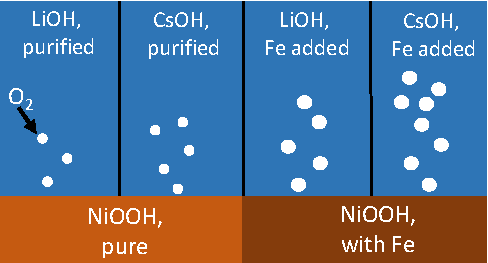
\includegraphics[width=.9\linewidth]{./images/toc.pdf}
% Emacs 25.1.50.1 (Org mode 8.2.10)
\end{document}